\newcommand{\GammaBar}{\overline{\BG}}
\newcommand{\GBar}{\overline{G}}
\newcommand{\CBar}{\overline{C}}
\newcommand{\VBGBar}{\overline{\vb G}}
\newcommand{\VBCBar}{\overline{\vb C}}
\newcommand{\KB}{\vb k\subt{B}}

%%%%%%%%%%%%%%%%%%%%%%%%%%%%%%%%%%%%%%%%%%%%%%%%%%%%%%%%%%%%%%%%%%%%%
%%%%%%%%%%%%%%%%%%%%%%%%%%%%%%%%%%%%%%%%%%%%%%%%%%%%%%%%%%%%%%%%%%%%%
%%%%%%%%%%%%%%%%%%%%%%%%%%%%%%%%%%%%%%%%%%%%%%%%%%%%%%%%%%%%%%%%%%%%%
\section{BEM formulations for PBC bodies}

%=================================================
%=================================================
%=================================================
\subsection{Scattered field of an infinite PEC surface}

Consider the scattered field produced by an 
induced surface-current density $\vb K(\vb x)$ on
an infinite PEC surface $\mc S_\infty$:
%====================================================================%
\begin{align}
  \vb E\sups{scat}(\vb x)
&=
  \int_{\mc S_\infty} 
   \BG\supt{EE}(\vb x, \vb x^\prime)
   \cdot 
   \vb K(\vb x^\prime)d\vb x^\prime
\\
&=
  ikZ_0
  \int_{\mc S_\infty} 
   \vb G(\vb x, \vb x^\prime) 
   \cdot 
   \vb K(\vb x^\prime)d\vb x^\prime
\label{EScatPBC}
\end{align}
where $k=\omega/c$ ($\omega$ is the angular frequency
at which we are working) and $Z_0$ is the impedance
of free space (assume we are in vacuum for now).
If we now suppose that 
%====================================================================%
\begin{itemize}
 \item the surface $\mc S_\infty$ consists of an infinite lattice
       of copies of a unit-cell surface $\mc S_0$ translated through
       two-dimensional lattice vectors of the form 
       \numeq{LatticeVectors}{\vb L=n_1 \vb L_1 + n_2\vb L_2}
       and
 \item the surface current respects this periodicity in the 
       Bloch sense, i.e. we have
       \numeq{KPeriodicity}
       {\vb K(\vb x+\vb L)
          = e^{i\KB \cdot \vb L} \, \vb K(\vb x)
       }
       for some Bloch vector $\KB$
\end{itemize}
%====================================================================%
then I can write the scattered field (\ref{EScatPBC}) as an integral
over just the unit cell:
%====================================================================%
\begin{align}
   \vb E\sups{scat}(\vb x)
&= ikZ_0 
   \sum_{\vb L}
   \int_{\mc S_0}
   \vb G(\vb x, \vb x^\prime+\vb L)
   \cdot 
   \vb K(\vb x^\prime + \vb L ) \, d\vb x^\prime
\nn
&= ikZ_0
   \int_{\mc S_0}
   \underbrace{
   \left\{
   \sum_{\vb L}
   e^{i\KB \cdot \vb L}
   \vb G(\vb x, \vb x^\prime+\vb L)
   \right\}
              }_{\VBGBar(\vb x, \vb x^\prime)}
   \cdot 
   \vb K(\vb x^\prime) \, d\vb x^\prime
\nn
&= ikZ_0 
   \int_{\mc S_0}
   \VBGBar(\vb x, \vb x^\prime)
   \cdot 
   \vb K(\vb x^\prime) \, d\vb x^\prime
\label{EScatPBC}
\end{align}
where $\VBGBar$ is the dyadic periodic Green's function,
whose properties we now discuss.

%%%%%%%%%%%%%%%%%%%%%%%%%%%%%%%%%%%%%%%%%%%%%%%%%%%%%%%%%%%%%%%%%%%%%%
%%%%%%%%%%%%%%%%%%%%%%%%%%%%%%%%%%%%%%%%%%%%%%%%%%%%%%%%%%%%%%%%%%%%%%
%%%%%%%%%%%%%%%%%%%%%%%%%%%%%%%%%%%%%%%%%%%%%%%%%%%%%%%%%%%%%%%%%%%%%%
\subsection{Periodic Green's functions}

The dyadic periodic Green's function introduced in 
(\ref{EScatPBC}) is 
%====================================================================%
\begin{align*}
 \VBGBar(\vb x, \vb x^\prime)
&=\sum_{\vb L} e^{i\KB \cdot \vb L}\vb G(\vb x, \vb x^\prime+\vb L)
\\
 \VBGBar(\vb x, \vb x^\prime)
&=\sum_{\vb L} e^{i\KB \cdot \vb L}\vb G(\vb x-\vb x^\prime-\vb L)
\intertext{with cartesian components}
 \GBar_{ij}(\vb x, \vb x^\prime)
&=\sum_{\vb L} e^{i\KB \cdot \vb L}G_{ij}(\vb x-\vb x^\prime-\vb L)
\\
&=\sum_{\vb L} 
   e^{i\KB \cdot \vb L} 
  \left[
   \Big( \delta_{ij} + \frac{1}{k^2}\partial_i \partial_j\Big)
   \frac{e^{ik|\vb x - \vb x^\prime - \vb L|}}
        {4\pi|\vb x - \vb x^\prime - \vb L|}
  \right]
\intertext{Interchange differentiation and summation:}
&=
  \Big( \delta_{ij} + \frac{1}{k^2}\partial_i \partial_j\Big)
  \underbrace{
  \left\{ \sum_{\vb L} 
          e^{i\KB \cdot \vb L}
          \frac{e^{ik|\vb x - \vb x^\prime - \vb L|}} 
          {4\pi|\vb x - \vb x^\prime - \vb L |}
   \right\}}_{\GBar_0(\vb x-\vb x^\prime)}
\end{align*}
where $\GBar_0$ is the scalar periodic Green's function.
(\lss computes $\GBar_0$ and its derivatives using Ewald
summation together with an interpolation-table method
discussed below.)
%====================================================================%

I will also need the periodic version of the $\vb C$ dyadic
(or ``MFIE kernel''),
%====================================================================%
\begin{align*}
  \VBCBar(\vb x, \vb x^\prime)
 &=\sum_{\vb L} e^{i\KB \cdot \vb L}\vb C(\vb x-\vb x^\prime-\vb L)
\intertext{with components}
  \CBar_{ij}(\vb x, \vb x^\prime)
 &=\sum_{\vb L} e^{i\KB \cdot \vb L}C_{ij}(\vb x-\vb x^\prime-\vb L)
\\
 &=\frac{1}{ik}\epsilon_{ij\ell} \partial_\ell 
   \sum_{\vb L} e^{i\KB \cdot \vb L}G_0(\vb x-\vb x^\prime-\vb L).
\end{align*}
%====================================================================%

\paragraph{Transpositional symmetries of periodic Green's functions}

The non-periodic $\vb G$ and $\vb C$ dyadics are invariant 
under simultaneous transposition of indices and inversion of 
argument:
%--------------------------------------------------------------------%
\numeq{GCTranspose}
{
  G_{ij}(\vb r) = G_{ji}(-\vb r), \qquad 
  C_{ij}(\vb r) = C_{ji}(-\vb r).
}
%--------------------------------------------------------------------%
Now consider the implications of this for the periodic dyadics. In
particular, we write
%--------------------------------------------------------------------%
\begin{subequations}
\begin{align}
  \GBar_{ij}(\KB; \vb x, \vb x^\prime)
 &=\sum_{\vb L} e^{i\KB \cdot \vb L}G_{ij}(\vb x-\vb x^\prime-\vb L)
\nonumber
\intertext{Use (\ref{GCTranspose}):}
 &=\sum_{\vb L} e^{i\KB \cdot \vb L}G_{ji}(\vb x^\prime-\vb x^\prime+\vb L)
\nonumber
\intertext{Relabel the summation variable according to $\vb L \to -\vb L$:}
 &=\sum_{\vb L} e^{-i\KB \cdot \vb L}G_{ji}(\vb x^\prime-\vb x-\vb L)
\nn
 &=\GBar_{ji}(-\KB; \vb x^\prime, \vb x)
\intertext{and similarly}
  \CBar_{ij}(\KB; \vb x, \vb x^\prime)
&=\CBar_{ji}(-\KB; \vb x^\prime, \vb x).
\end{align}
\label{TranspositionSymmetries}
\end{subequations}
%--------------------------------------------------------------------%
Thus the periodic $\vb G$ and $\vb C$ dyadics are invariant
under simultaneous transposition of indices, interchange of 
$\vb x,\vb x^\prime$, and inversion of the Bloch vector.

\paragraph{Translational symmetries of periodic Green's functions}

Suppose the lattice basis vectors are $\vb L_1, \vb L_2$.
Then we can write the sum that defines the scalar periodic Green's
function in the form
%====================================================================%
\begin{align*}
\GBar_0(\vb r)
&= \sum_{n_1, n_2=-\infty}^\infty 
   e^{i\KB \cdot(n_1 \vb L_1 + n_2 \vb L_2)}
     G_0(\vb r - n_1\vb L_1 - n_2 \vb L_2)
\end{align*}
%====================================================================%
Now consider evaluating $\GBar$ at an argument displaced
through one full lattice basis vector:
\begin{align*}
 \VBGBar(\vb r + \vb L_1) 
&= \sum_{n_1, n_2=-\infty}^\infty 
   e^{i\KB \cdot (n_1\vb L_1 + n_2\vb L_2)}
   G_0( \vb r + \vb L_1 - n_1 \vb L_1 - n_2 \vb L_2)
\intertext{Add and subtract $\vb L_1$ in the exponent of 
           the Bloch factor:}
&= e^{i\KB \cdot \vb L_1}
   \sum_{n_1, n_2=-\infty}^\infty 
   e^{i\KB \cdot [(n_1-1)\vb L_1 + n_2\vb L_2]}
   G_0( \vb r -(n_1-1)\vb L_1 - n_2 \vb L_2)
\intertext{Now just redefine $n_1\to n_1-1$ in the infinite sum:}
&= e^{i\KB \cdot \vb L_1} \VBGBar( \vb r ).
\end{align*}
%====================================================================%
More generally, for any lattice vector $\vb L$ I have
$$
 \VBGBar(\vb r + \vb L)
 = e^{i\KB \cdot \vb L}\VBGBar(\vb r).
$$

%=================================================
%=================================================
%=================================================
\subsection{Discretized EFIE formulation}

Now consider solving for $\vb K(\vb x)$ in the presence
of illumination by an external Bloch-periodic 
field $\vb E\sups{inc}$.
We suppose that the current distribution in the unit cell 
is represented approximately by an expansion in basis
functions $\{\vb b_\alpha(\vb x)\}:$
%====================================================================%
\numeq{KExpansionPBC}
{\vb K(\vb x) \approx k_\alpha \vb b_\alpha(\vb x).}
%====================================================================%
The electric-field integral equation reads
%====================================================================%
\numeq{EFIE}
{\vb E\sups{scat}_\parallel(\vb x)
   =-\vb E\sups{inc}_\parallel(\vb x).
}
%====================================================================%
As in the usual compact-surface case, inserting (\ref{EScatPBC}) 
and (\ref{KExpansionPBC}) and testing with each element in the set 
$\{\vb b_\alpha\}$ yields a discretized PBC EFIE:
%====================================================================%
\begin{align}
 \sum_{\beta}
 \underbrace{
   \Big \langle \vb b_\alpha \Big|
   ikZ_0\VBGBar    
   \Big| \vb b_\beta \Big\rangle
            }_{\vb M_{\alpha\beta}} 
   k_\beta
&=-\Big \langle \vb b_\alpha \Big | \vb E\sups{inc} \Big\rangle
\label{PBCEFIE}
\end{align}
%====================================================================%
In other words, we obtain a formulation that looks exactly
like the formulation for compact objects, with the only
difference being that the elements of the BEM matrix
involve the $\VBGBar$ kernel in place of the usual 
$\vb G$ dyadic Green's function.

Note that the testing procedure that leads to 
(\ref{PBCEFIE}) is only testing the satisfaction
of equation (\ref{EFIE}) for points $\vb x$
\textit{in the unit cell.} However, the Bloch-periodicity
of the incident and scattered fields ensures that
satisfaction of the equation throughout the unit cell
implies its satisfaction everywhere.

%=================================================
%=================================================
%=================================================
\subsection{Symmetries of the PBC BEM matrix}

For a PEC structure, the $\alpha,\beta$ element of 
the BEM matrix is 
%--------------------------------------------------------------------%
\begin{align*}
 M_{\alpha\beta}(\KB)
&= ik\Big \langle \vb b_\alpha \Big|
    \VBGBar(\KB)
   \Big| \vb b_\beta \Big\rangle
\\
&= ik\int 
   \Big\{ 
   b_{\alpha i}(\vb x_\alpha) 
   \underbrace{\GBar_{ij}(\KB; \vb x_\alpha , \vb x_\beta)}
             _{=\GBar_{ji}(-\KB; \vb x_\beta , \vb x_\alpha )}
   b_{\beta j}(\vb x_\beta) 
   \Big\}\, d\vb x_\alpha d\vb x_\beta
\\
&= ik\Big \langle \vb b_\beta\Big|
    \VBGBar(-\KB)
   \Big| \vb b_\alpha\Big\rangle
\\
&=M_{\beta\alpha}(-\KB)
\end{align*}
%--------------------------------------------------------------------%
where we used equation (\ref{TranspositionSymmetries}a). 
For a dielectric structure, the matrix elements also involve
inner products with $\VBCBar$ dyadics, but since $\VBCBar$ satisfies
the same symmetry as $\VBGBar$ (\ref{TranpositionSymmetry}b), 
a similar equation holds in that case.

Thus in general for both PEC and non-PEC BEM matrices we have
\numeq{PBCMatrixTranspose}
{\vb M(\KB) = \Big[ \vb M(-\KB) \Big]^T}
where $T$ denotes the \textit{non-conjugate} transpose.

\subsubsection*{Symmetries in the imaginary frequency case}

For equilibrium Casimir computations we need elements
of the BEM matrix at imaginary frequencies. 
%====================================================================%
$$ \vb M(i\xi, \KB) = \vb M(i\xi, \KB)^\dagger $$
%====================================================================%

%%%%%%%%%%%%%%%%%%%%%%%%%%%%%%%%%%%%%%%%%%%%%%%%%%%%%%%%%%%%%%%%%%%%%%
%%%%%%%%%%%%%%%%%%%%%%%%%%%%%%%%%%%%%%%%%%%%%%%%%%%%%%%%%%%%%%%%%%%%%%
%%%%%%%%%%%%%%%%%%%%%%%%%%%%%%%%%%%%%%%%%%%%%%%%%%%%%%%%%%%%%%%%%%%%%%
\section{PBC geometries in {\sc scuff-em}}

%=================================================
%=================================================
%=================================================
\subsection{Overview}

\lss supports Bloch-periodic boundary conditions for
periodically repeated geometries. In this case,

\begin{itemize}
 \item The \texttt{.scuffgeo} file will contain
       a \texttt{LATTICE...ENDLATTICE} section defining 
       between one and three lattice basis vectors 
       $\vb L_1, \vb L_2, \vb L_3.$ (In the present 
       discussion we will consider the common case
       of two-dimensional periodicity, so we have two
       lattice basis vectors $\vb L_1, \vb L_2$.) 
       We assume that $\vb L_1, \vb L_2$ have no 
       component in the $z$ direction.
 \item The only portion of the geometry that is
       meshed is that contained with the ``unit cell.''
 \item We will refer to the lattice cell obtained by 
       displacing the unit cell through displacement 
       vector $\vb L=n_1 \vb L_1 + n_y \vb L_2$ as 
       ``lattice cell $(n_1, n_2)$'' or sometimes
       ``lattice cell $\vb L$''.
 \item All currents and fields in lattice cell $(n_1,n_2)$
       are understood to be equal to the corresponding
       currents and fields in lattice cell $(0,0)$ times
       a Bloch phase factor $e^{i\KB \cdot \vb L}$ where
       $\KB$ is the Bloch wavevector.
\end{itemize}

%=================================================
%=================================================
%=================================================
\subsection{Straddlers}

Suppose we are trying to mesh the unit cell
of a square-lattice geometry.
Consider the square mesh shown in the 
upper portion of Figure \ref{NoStraddlerFigure}.
If \lss were given this mesh as a description of a
\textit{compact} surface, it would assign a 
total of 40 basis functions, as indicated by 
the arrows in the lower portion of 
Figure \ref{NoStraddlerFigure}.
In particular, no basis functions would be assigned
to exterior edges. Such a set of basis functions
would have the property that, when we consider
the infinite surface obtained by periodically
replicating the mesh and the basis functions,
no currents could flow from one unit cell to the next;
all currents would be localized within the area of
individual unit cells. 
%####################################################################%
\begin{figure}
\begin{center}
\begin{tabular}{c}
\resizebox{!}{0.5\textheight}{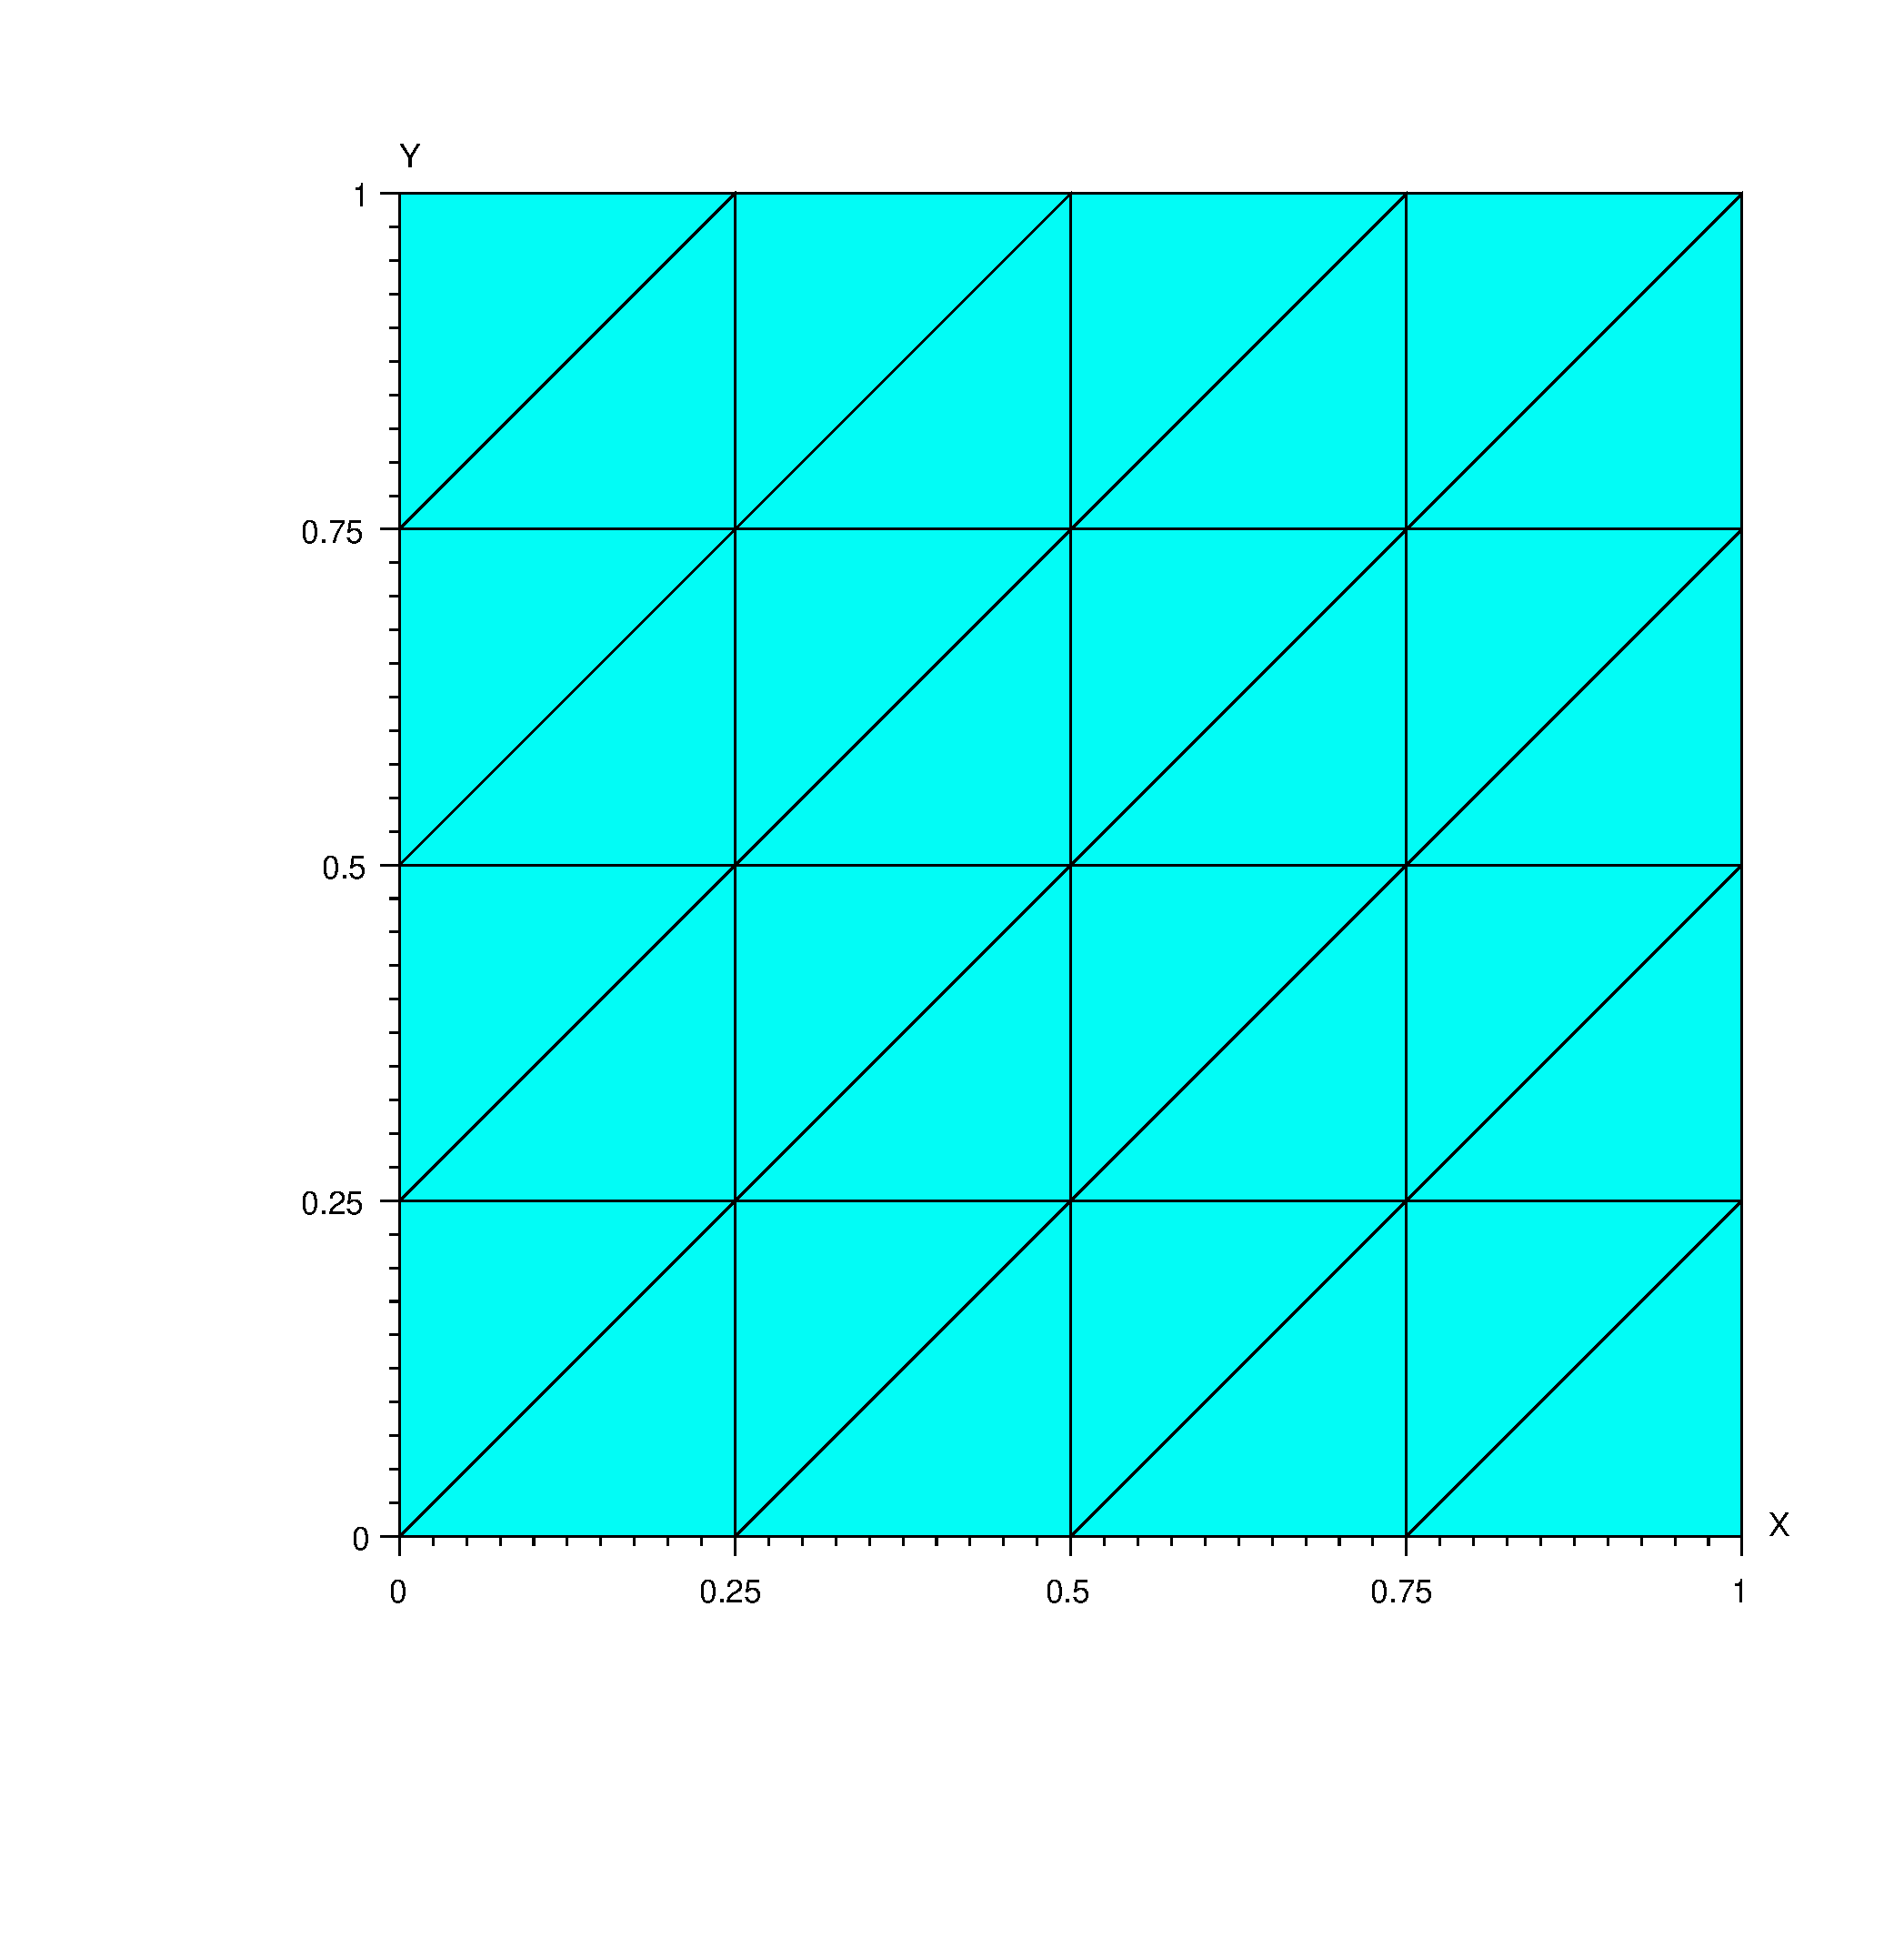
\includegraphics{SquareMesh0.pdf}}
\\[-0.5in]
\hspace{0.45in} \resizebox{!}{0.05\textheight}{$\Downarrow$}
\\[-0.2in]
\resizebox{!}{0.5\textheight}{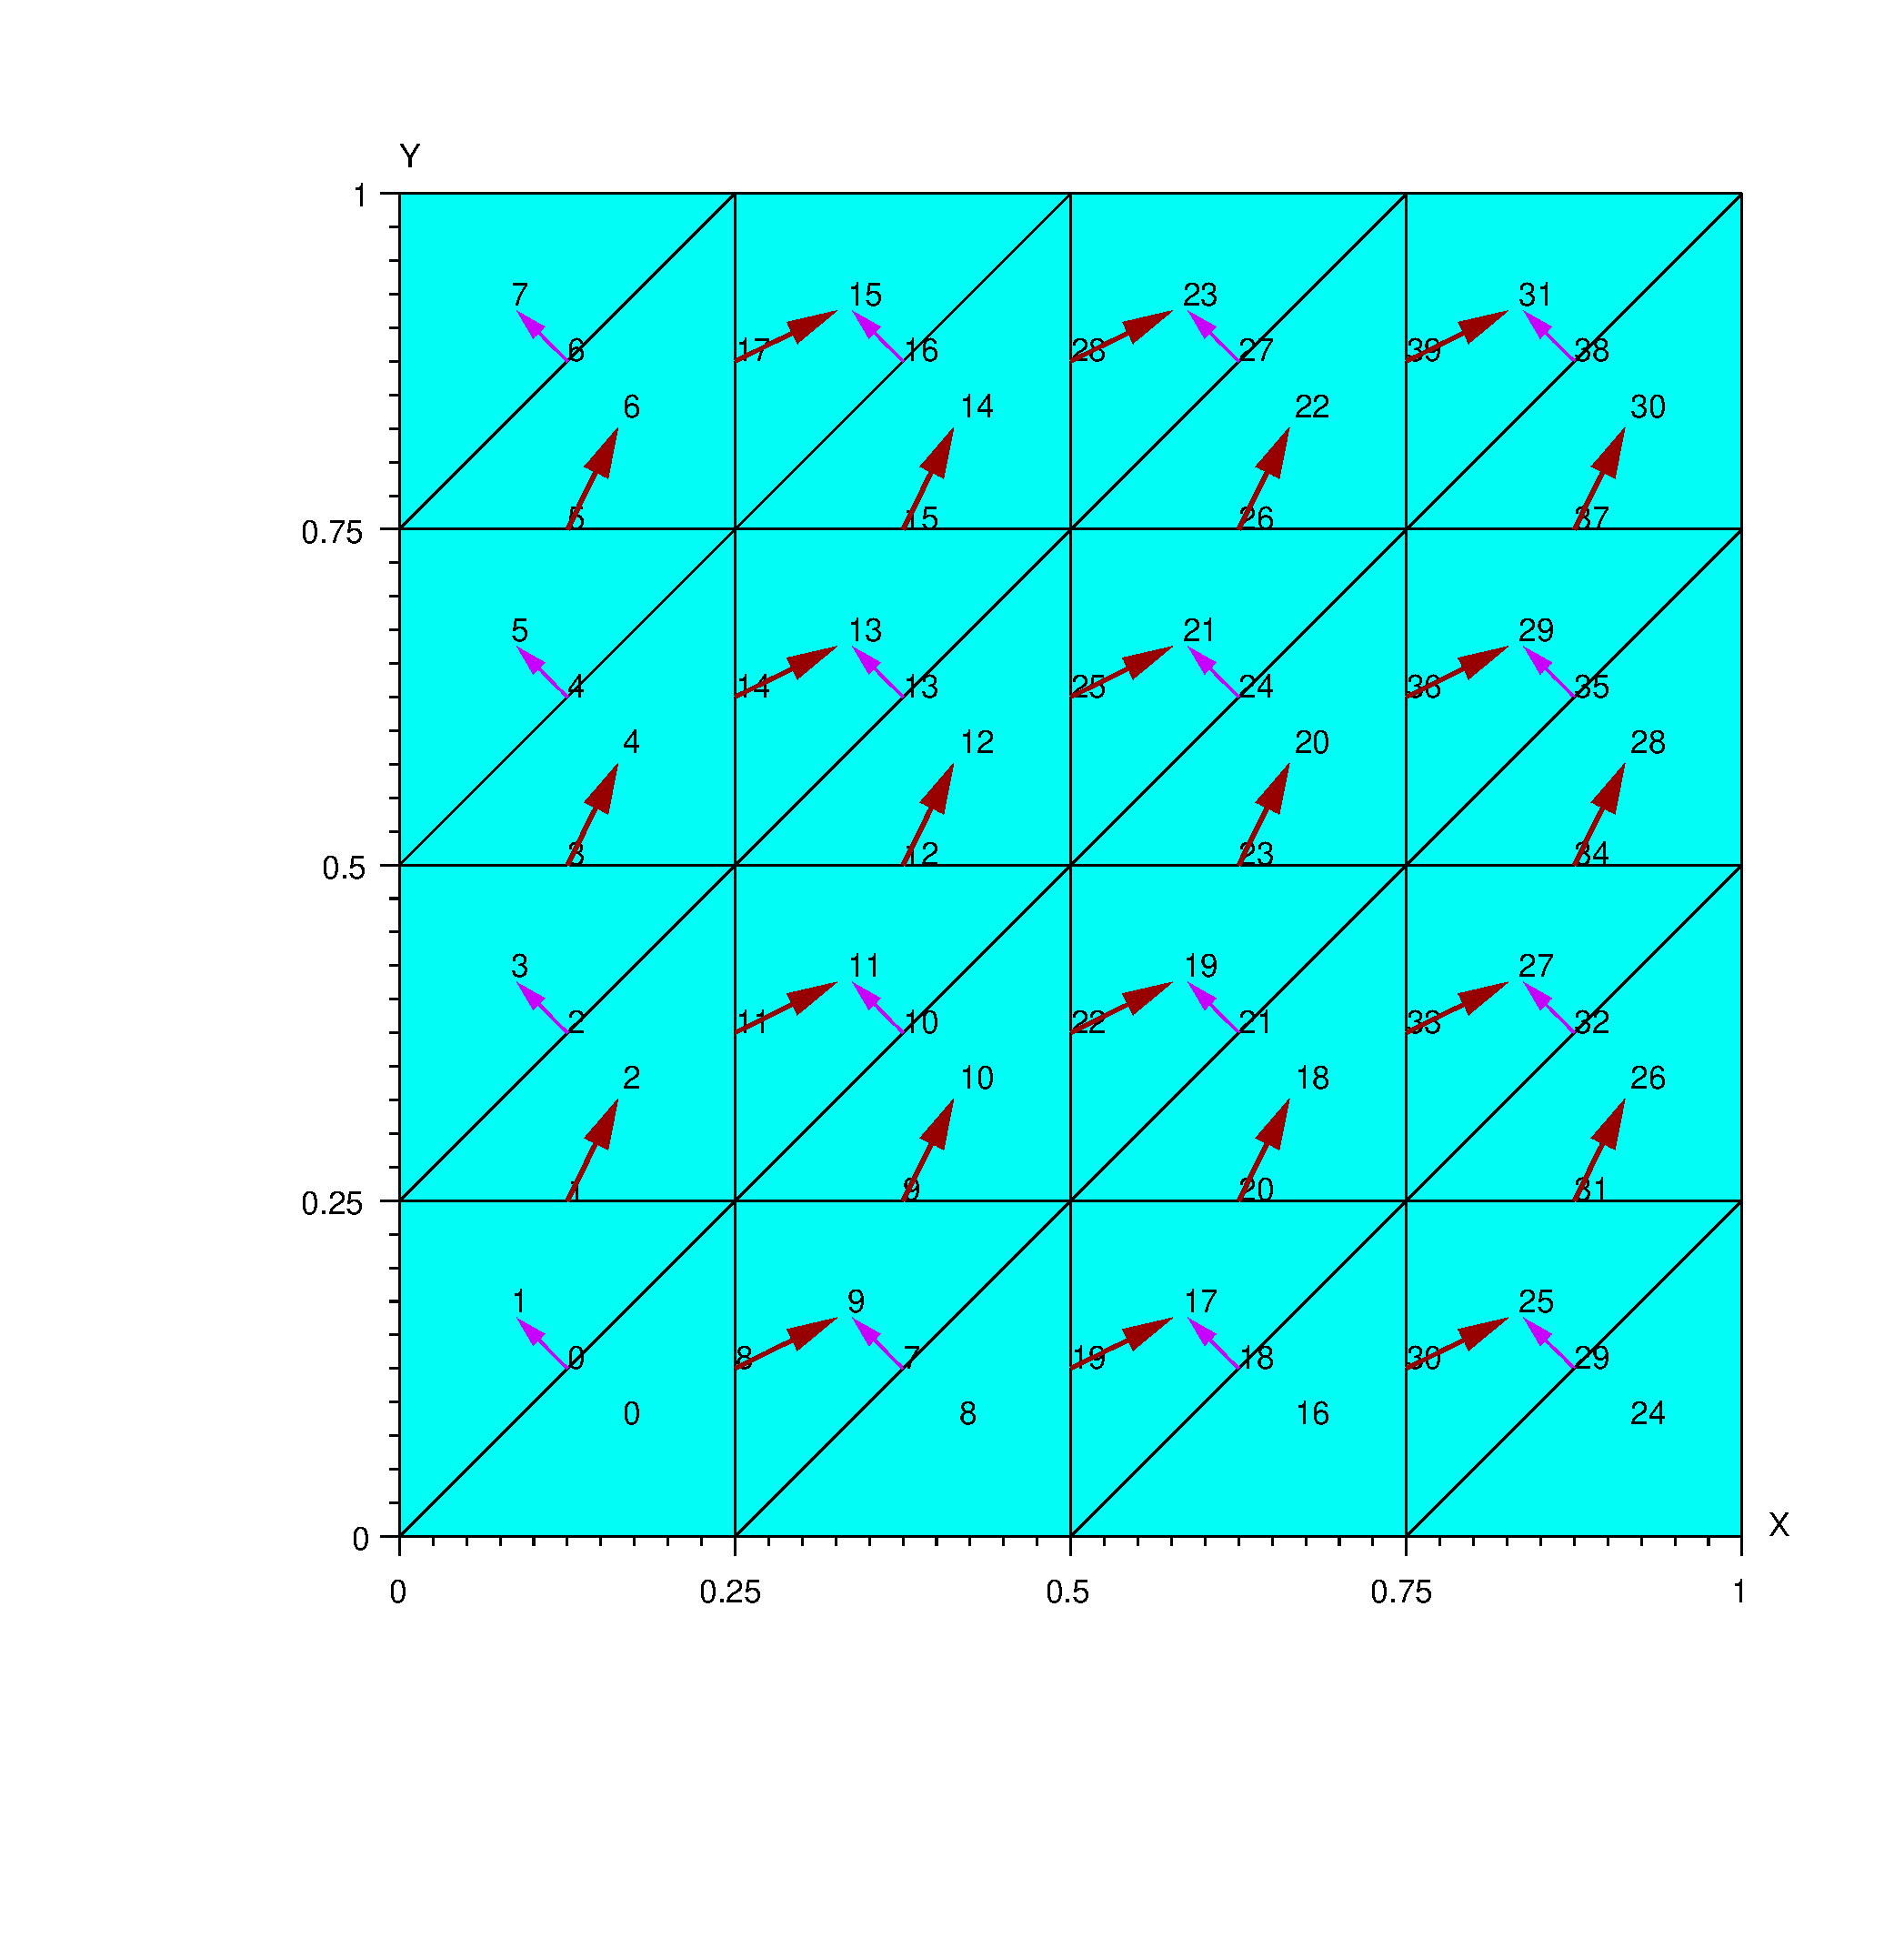
\includegraphics{SquareMesh1.pdf}}
\end{tabular}
\caption{The usual assignment of RWG basis functions 
         to an input surface mesh.
         Integers inside panels denote panel indices.
         Indices lying atop edges denote RWG basis-function indices.
         Arrows indicate directions of current flow.
        } 
\label{NoStraddlerFigure}
\end{center}
\end{figure}
%####################################################################%
To remedy this difficulty, \lss automatically
adds \textit{straddlers} to the surface meshes
specified to the code in geometries involving
extended surfaces. 
This is illustrated in Figure \ref{StraddlerFigure}.
%####################################################################%
\begin{figure}
\begin{center}
\resizebox{\textwidth}{!}{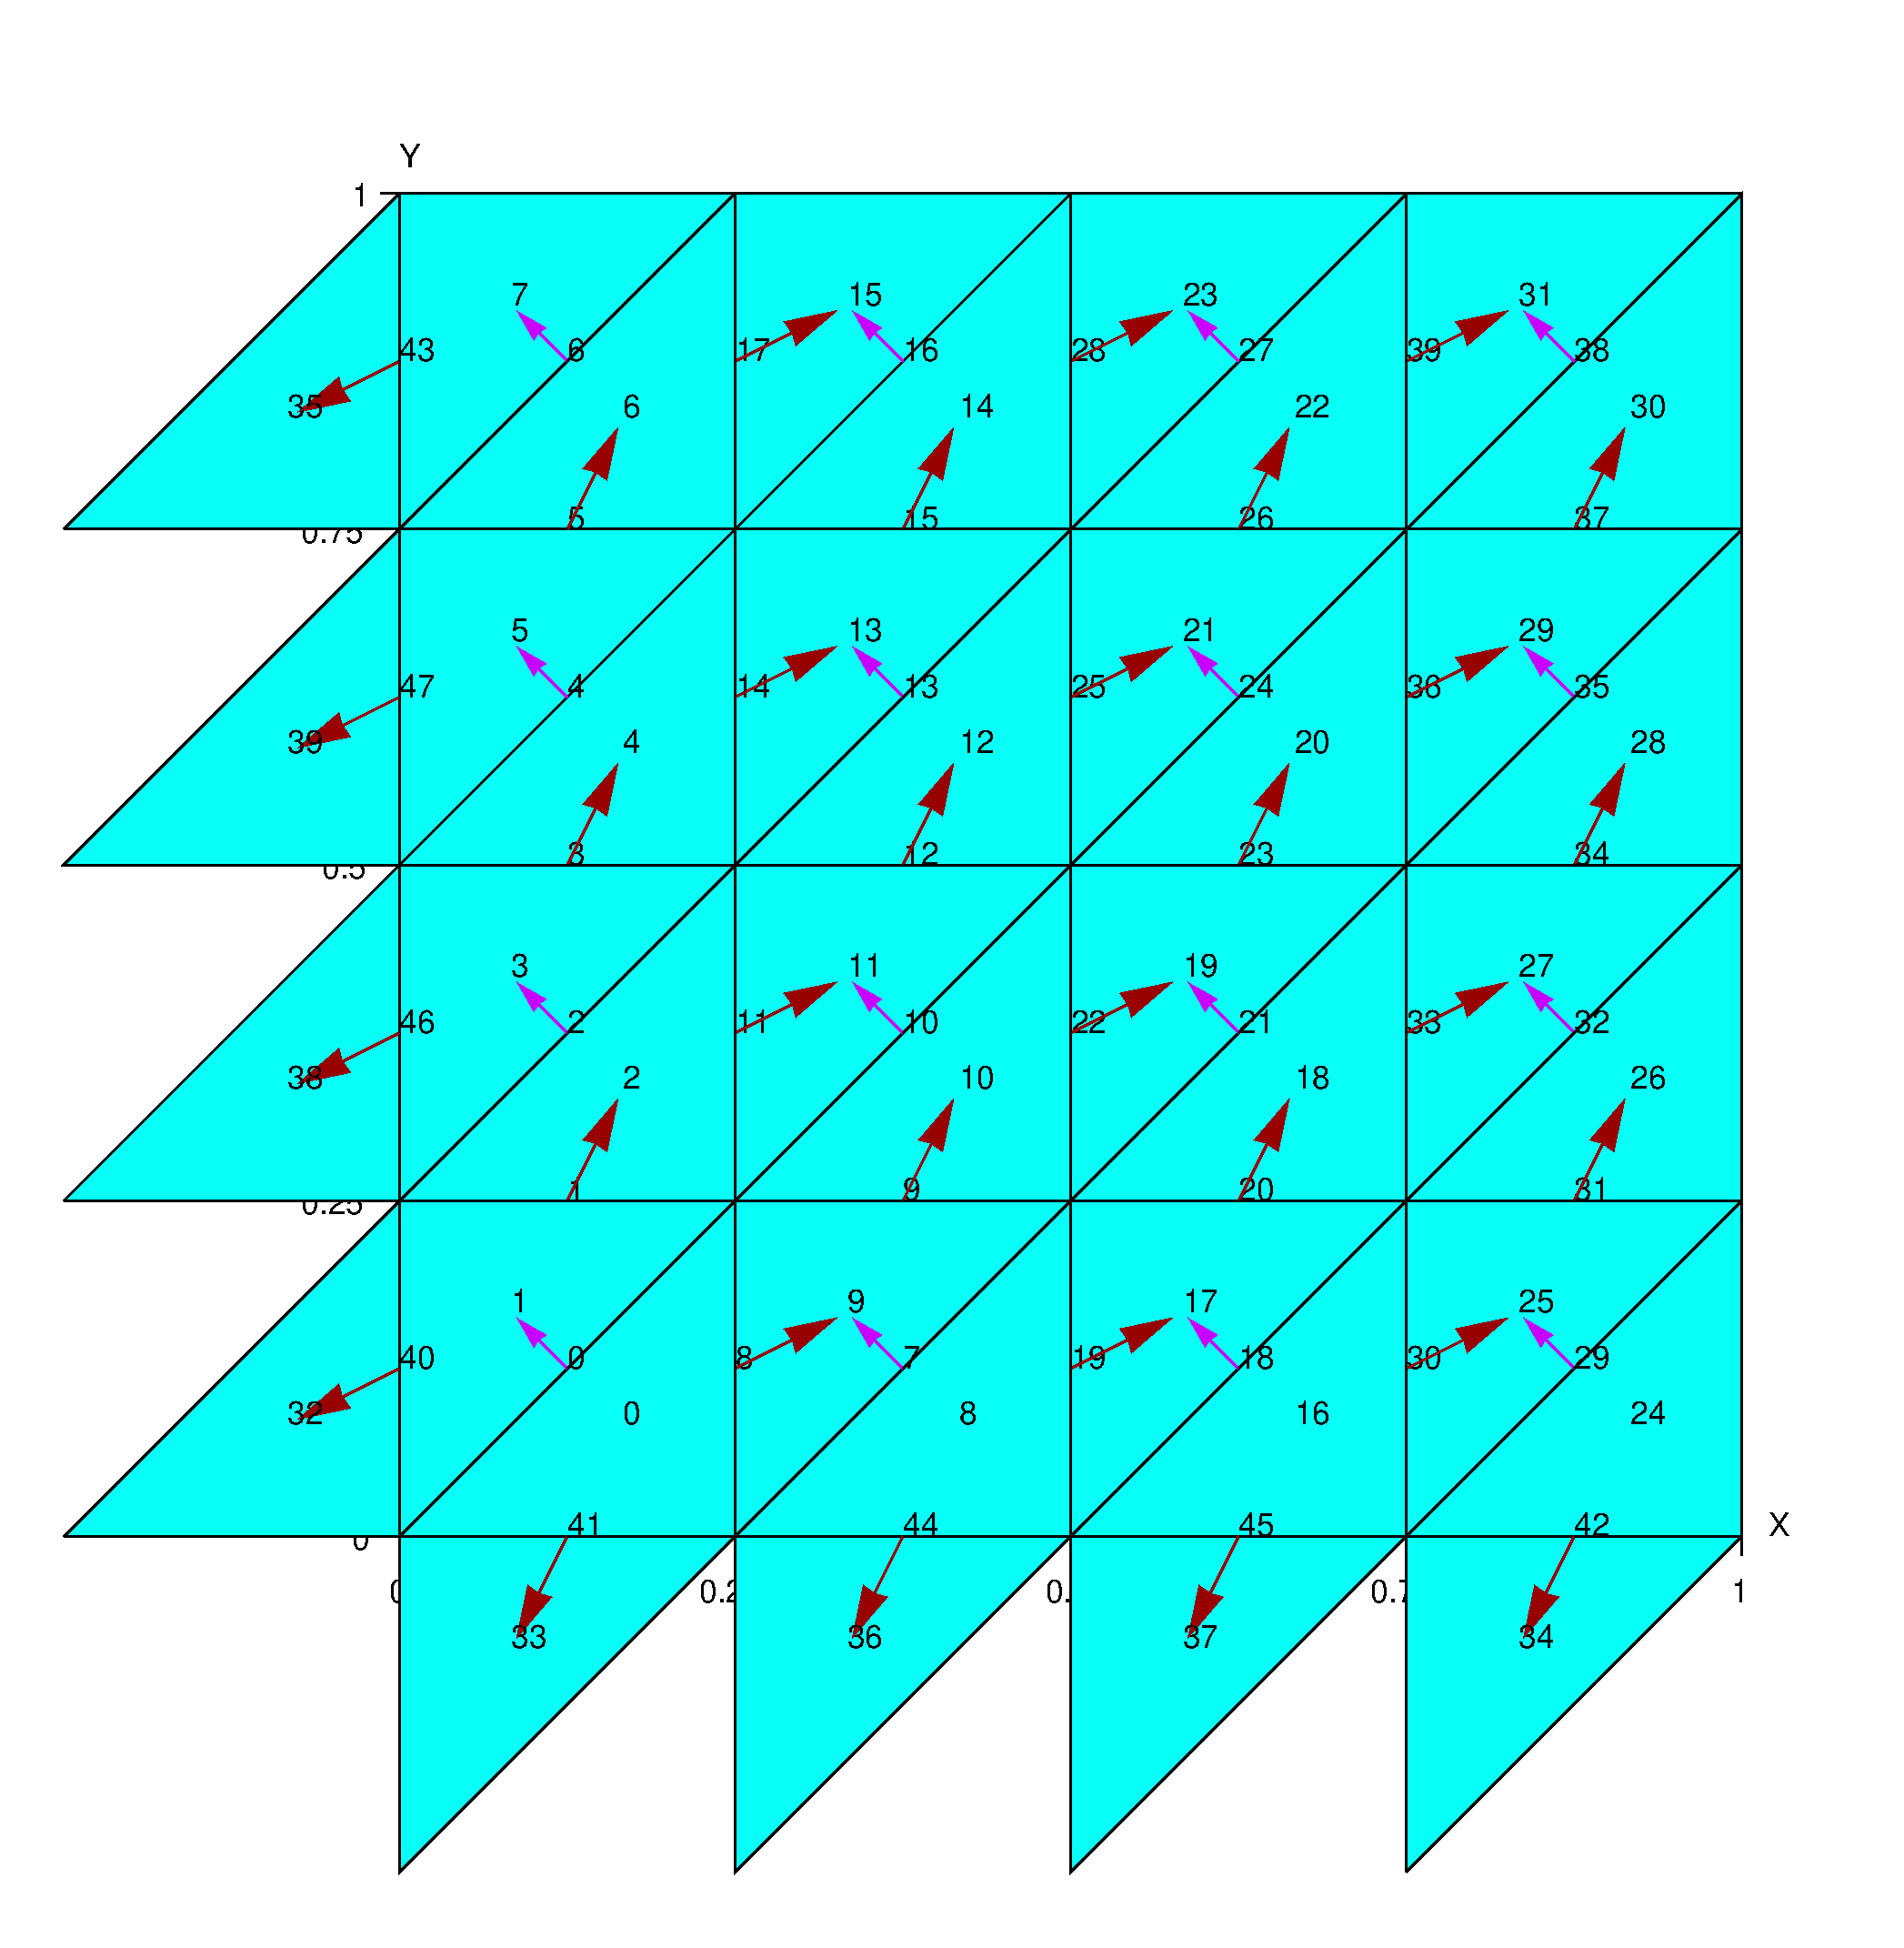
\includegraphics{SquareMesh2.pdf}}
\caption{Straddlers. 
         Integers inside panels denote panel indices.
         Indices lying atop edges denote RWG basis-function indices.
         Arrows indicate directions of current flow.}
\label{StraddlerFigure}
\end{center}
\end{figure}
%####################################################################%

%=================================================
%=================================================
%=================================================
\subsection{Evaluation of surface currents within the unit cell}

When evaluating the $\vb K$ and $\vb N$ surface-current 
distributions at panels that border the upper or right edges 
of the unit-cell mesh, we have to be careful to account for the 
contribution of straddlers. 

For example, consider evaluating the electric surface current at 
oints $\vb x$ inside panel $\mc P_{24}$ in Figure \ref{StraddlerFigure}.
There are three RWG basis functions that contribute to the current
at this point: the functions associated with edges 29 and 42,
and the periodic image of the function associated with edge 40.
Thus we compute
%====================================================================%
$$ \vb K(\vb x) 
   =   k_{29} \vb b_{29}(\vb x) + k_{42} \vb b_{42}(\vb x) 
     + e^{i \KB \cdot \vb L_1} k_{40} \vb b_{40}(\vb x-\vb L_1)
$$
%====================================================================%
where $\vb L_1$ is the lattice basis vector through which we
translate points in panel 32 to yield points in panel 24.
[In this case we have $\vb L_1=(1,0).$]

%=================================================
%=================================================
%=================================================
\subsection{Relations between BEM matrix elements}

Looking at Figure \ref{StraddlerFigure}, it seems 
obvious that BEM matrix elements between the pair of 
basis functions
$\{\vb b_2, \vb b_{24}\}$ will be identical to those
between the pair 
$\{\vb b_4, \vb b_{27}\}$. (This much would be 
true even if we \textit{weren't} talking about
periodic geometries.)

Slightly less obvious is that matrix elements between
the pair $\{\vb b_6, \vb b_{18}\}$ will \textit{also}
be related to matrix elements between the above two
pairs---in fact, the elements will be \textit{identical}
for $\KB=0$ and will differ by only a phase factor
for $\KB\ne 0$. Let's now derive this relationship.

Let $\vb L$ be a lattice vector and 
let 
$\{\vb b_{\alpha}, \vb b_{\beta}\}$
and 
$\{\vb b_{\alpha^\prime}, \vb b_{\beta^\prime}\}$ 
be two pairs of RWG basis functions for which the 
displacement between centroids differs by $\vb L$.
That is, we have 
$$ \vb x_{0\beta}-\vb x_{0\alpha}
   =
   \vb x_{0\beta^\prime}-\vb x_{0\alpha^\prime} + \vb L
$$
where e.g. $\vb x_{0\beta}$ denotes the centroid of 
the support of $\vb b_\beta$.
Examples of basis-function pairs in the mesh of 
Figure \ref{StraddlerFigure} for which this condition
is satisfied include
$$\begin{array}{lclclclclcl}
  (\alpha,\beta)&=&(4,27),  
  &\qquad
  (\alpha^\prime,\beta^\prime)&=&(6,18), 
  &\qquad
  \vb L &=& (0,1)
\\[5pt]
  (\alpha,\beta)&=&(0,32),
  &\qquad
  (\alpha^\prime,\beta^\prime)&=&(7,2), 
  &\qquad
  \vb L &=& (1,0).
  \end{array}
$$

%=================================================
%=================================================
%=================================================
\subsection{Assembly of BEM matrix blocks}

For a geometry in which the unit cell contains $N$ 
surfaces, the BEM matrix at Bloch wavevector $\KB$ 
has the structure
%====================================================================%
\numeq{BlockMatrixStructure}
{ \vb M(\KB)
 =\left(\begin{array}{cccc}
  \vb T_1(\KB)    & \vb U_{12}(\KB) & \cdots & \vb U_{1N}(\KB) \\[3pt]
  \vb U_{21}(\KB) & \vb T_2(\KB)    & \cdots & \vb U_{2N}(\KB) \\[3pt]
  \vdots          & \vdots          & \ddots & \vdots      \\[3pt]
  \vb U_{N1}(\KB) & \vb U_{N2}(\KB) & \cdots & \vb T_{N}(\KB)
  \end{array}\right)
}
%====================================================================%
where $\vb U_{mn}$ describes the interaction of surfaces $m$
and $n$ and $\vb T_m$ describes the self-interaction of
surface $m$.

\subsubsection*{Off-diagonal blocks}

The off-diagonal blocks have the structure

%--------------------------------------------------------------------%
\begin{align}
\vb U_{mn}(\KB)
 =   &\vb U_{mn}\supt{00}
\label{UmnDecomposition}\\
   & + e^{ i \KB \cdot \vb L_1} \vb U_{mn}^{+0}
     + e^{-i \KB \cdot \vb L_1} \vb U_{mn}^{-0}
\nn
   & + e^{ i \KB \cdot \vb L_2} \vb U_{mn}^{0+}
     + e^{-i \KB \cdot \vb L_2} \vb U_{mn}^{0-}
\nn
   & + e^{ i \KB \cdot (\vb L_1+\vb L_2)} \vb U_{mn}^{++}
     + e^{-i \KB \cdot (\vb L_1+\vb L_2)} \vb U_{mn}^{--}
\nn
   & + e^{ i \KB \cdot (\vb L_1-\vb L_2)} \vb U_{mn}^{+-}
     + e^{-i \KB \cdot (\vb L_1-\vb L_2)} \vb U_{mn}^{-+}
\nn
   & + \vb U_{mn}\supt{AB9}(\KB).
\nonumber
\end{align}
%--------------------------------------------------------------------%
In this equation, $\vb U_{mn}^{\sigma \sigma^\prime}$ is the usual 
(non-periodic) matrix describing the interaction of surface $m$ 
with a \textit{displaced} copy of surface $n$; the displacement 
is through displacement vector $\sigma \vb L_1 + \sigma^\prime \vb L_2$
where $\sigma,\sigma^\prime \in \{-1,0,1\}.$ 
On the other hand, $\vb U_{mn}\supt{AB9}$ represents the interaction
of surface $m$ with the infinite set of Bloch-phased 
and displaced copies of surface $n$ \textit{excluding} the contribution
of the innermost 9 grid cells (``AB9'' stands for ``all but 9.'')

The point of the decomposition (\ref{UmnDecomposition}) is that 
the matrix blocks $\vb U_{mn}^{\sigma\sigma^\prime}$ are 
\textit{independent of $\KB$} and hence need only be computed 
once at a given angular frequency, after which they may be reused
for any number of calculations at different points in the Brillouin
zone. 

In {\sc scuff-em}, the $\KB$-independent matrix blocks 
$\vb U_{mn}^{\sigma\sigma^\prime}$ are computed using the ordinary
algorithm for assembling the blocks of the BEM matrix 
for compact (non-periodic) geometries. An advantage of this
is that singular integrals involving pairs of panels in
adjacent cells with common edges or vertices are handled
correctly using singular-integral evaluation techniques
present in {\sc scuff-em}.
For example, in the mesh of Figure \ref{StraddlerFigure},
panel 1 of the unit-cell mesh has a common edge 
with panel 24 of the $(-1,0)$ mesh image.

\subsubsection*{Transposes of off-diagonal blocks}

Once we have computed the 
$\vb U_{mn}^{\sigma\sigma^\prime}$ blocks for the $mn$ block of 
the BEM, we may re-use them to compute the $nm$ block, as follows 
based on equation (\ref{PBCMatrixTranspose}):
%--------------------------------------------------------------------%
\begin{align}
\vb U_{nm}(\KB) 
=  &\Big[\vb U_{mn}(-\KB)\Big]^T 
\\
=  &\Big[\vb U_{mn}\supt{00}]^T
\\
   & + e^{ -i \KB \cdot \vb L_1} \Big[\vb U_{mn}^{+0}\Big]^T
     + e^{  i \KB \cdot \vb L_1} \Big[\vb U_{mn}^{-0}\Big]^T
\nn
   & + e^{ -i \KB \cdot \vb L_2} \Big[\vb U_{mn}^{0+}\Big]^T
     + e^{ +i \KB \cdot \vb L_2} \Big[\vb U_{mn}^{0-}\Big]^T
\nn
   & + e^{ -i \KB \cdot (\vb L_1+\vb L_2)} \Big[\vb U_{mn}^{++}\Big]^T
     + e^{ +i \KB \cdot (\vb L_1+\vb L_2)} \Big[\vb U_{mn}^{--}\Big]^T
\nn
   & + e^{ -i \KB \cdot (\vb L_1-\vb L_2)} \Big[\vb U_{mn}^{+-}\Big]^T
     + e^{ +i \KB \cdot (\vb L_1-\vb L_2)} \Big[\vb U_{mn}^{-+}\Big]^T
\nn
   & + \vb U_{nm}\supt{AB9}(\KB).
\nonumber
\end{align}
%--------------------------------------------------------------------%

\subsubsection*{Diagonal blocks}

For the diagonal blocks there are additional symmetries, e.g.
$ \vb T_{m}^{--} = \Big[\vb T_{m}^{++}\Big]^T, $
and hence the equivalent of (\ref{UmnDecomposition}) reads 
%--------------------------------------------------------------------%
\begin{align}
\vb T_{m}(\KB)
 =   &\vb T_{m}\supt{00}
\label{TmDecomposition}\\
   & + e^{ i \KB \cdot \vb L_1} \vb T_{m}^{+0}
     + e^{-i \KB \cdot \vb L_1} \Big[\vb T_{m}^{+0}\Big]^T
\nn
   & + e^{ i \KB \cdot \vb L_2} \vb T_{m}^{0+}
     + e^{-i \KB \cdot \vb L_2} \Big[\vb T_{m}^{0+}\Big]^T
\nn
   & + e^{ i \KB \cdot (\vb L_1+\vb L_2)} \vb T_{m}^{++}
     + e^{-i \KB \cdot (\vb L_1+\vb L_2)} \Big[ \vb T_{m}^{++}\Big]^T
\nn
   & + e^{ i \KB \cdot (\vb L_1-\vb L_2)} \vb T_{m}^{+-}
     + e^{-i \KB \cdot (\vb L_1-\vb L_2)} \Big[ \vb T_{m}^{+-}\Big]^T
\nn
   & + \vb T_{m}\supt{AB9}(\KB).
\nonumber
\end{align}
%--------------------------------------------------------------------%
Hence to assemble $\vb T(\KB)$ we need only compute and
store 5 $\KB$-independent blocks $\vb T^{\sigma \sigma^\prime}$
instead of the 9 $\KB$-independent blocks required to assemble
$\vb U(\KB)$.

\subsubsection*{Assessing the connectivity of regions}

An important subtlety in the BEM matrix assembly for dielectric
geometries treated by the PMCHWT formulation concerns the question
of the ``extendedness'' or connectivity of material regions.

In general, the surfaces $m,n$ whose interaction is described
by the $\vb T_m$ and $\vb U_{mn}$ blocks in (\ref{BlockMatrixStructure}) 
will interact through one or two common \textit{regions} (material media).
(More specifically, $\vb T$ blocks will typically involve two common
regions, while $\vb U$ blocks will typically involve one common region.)

The BEM matrix elements


